% ---------------------------------------------------------------------------
\section{Results}
\label{sec:results}
% ---------------------------------------------------------------------------

\subsection{Exact recovery and the threshold}
\label{sec:recovery}

An exact implementation confirms Theorem~\ref{thm:window}. On rings whose merges satisfy
its isolation hypothesis ($n_0=2000$, $o_n=0.01$), without noise HyperCommon returns the
planted rings exactly at each of the 20 thresholds of our grid inside the window for
$k=8$ and the 22 inside it for $k=16$, and at no threshold outside it ($\Omega<0.98$).
With a fifth of the edges rewired, the mean $\Omega$ at the best threshold is still
$1.000$ for $k=16$ and $0.991$ for $k=8$. Without the third-pair test the same graphs
are never recovered exactly: the two edges of the wedge that crosses a merge have
commonality $J_u(1)$, at least every threshold of the window, so the pair rule admits
that wedge throughout it.

\begin{figure*}[t]
  \centering
  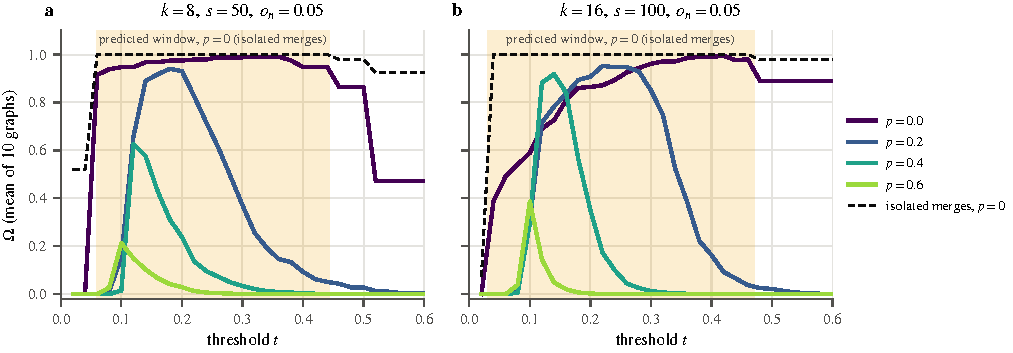
\includegraphics[width=\textwidth]{figures/fig_omega_t.pdf}
  \caption{Accuracy of HyperCommon as a function of the threshold on overlapping
  uniform rings ($n_0=2000$, $o_n=0.05$), one curve per rewiring level $p$, each the mean
  over ten test graphs. Shaded: the exact-recovery window that
  Theorem~\ref{thm:window} predicts for $p=0$ when merges are isolated; the plotted
  graphs' random merges do not satisfy the isolation hypothesis. Black dashed: graphs
  with isolated merges ($o_n=0.01$, merges more than $2k$ apart) at $p=0$, which reach
  $\Omega=1$ at every grid threshold inside the window and at none outside it.}
  \label{fig:omegat}
\end{figure*}

When merges fall at random they are rarely isolated: at $o_n=0.05$ a ring carries on
average at least as many merge positions as fit on it more than $k$ apart, and rings fuse through
nearby merged nodes (Proposition~\ref{prop:sharedpairs}). The noise-free curve still
stays between $0.92$ and $0.99$ across the window for $k=8$ [Fig.~\ref{fig:omegat}(a)].
As noise grows the best threshold moves down towards $t\approx0.1$, so the threshold has
to be chosen per graph. The overlapping modularity of the cover chooses it well: the
label-free threshold attains at least $95\%$ of the best threshold's mean $\Omega$ on 27
of the 36 benchmark settings and at least $90\%$ on 31 (Tables~\ref{tab:labelfree}
and~\ref{tab:oracle}).

\subsection{Planted rings}
\label{sec:planted}

\begin{table*}[t]
\caption{Scorecard of the benchmarks under the four protocols: $\Omega$ of HyperCommon minus that of the best other method (ablations excluded), mean over the noise range ($p\in[0,0.8]$ for rings, $\mu\in[0.1,0.6]$ for LFR), ten test graphs per noise level, with the best other method in brackets when HyperCommon is not significantly ahead of it and its difference rounds to 0.00 or below. Mark: the paired 95\% bootstrap interval of the difference over the ten test seeds lies above zero ($+$), contains zero ($=$) or lies below zero ($-$); intervals and the second-best method in Table~\ref{tab:S-intervals}. Oracle: best parameter per graph; label-free: largest overlapping modularity, Eq.~\eqref{eq:qov}; frozen: one parameter per family from calibration graphs; native: each method's own default or selection rule where it has one (Sec.~\ref{sec:protocol}), the label-free choice otherwise. Counts are not corrected for multiplicity. Method abbreviations as in Table~\ref{tab:labelfree}; the full tables are Tables~\ref{tab:labelfree} and~\ref{tab:oracle}--\ref{tab:native}.}
\label{tab:scorecard}
\scriptsize\setlength{\tabcolsep}{3pt}
\begin{ruledtabular}
\begin{tabular}{llcccc}
Family & $o_n$ & oracle & label-free & frozen & native \\
\hline
uniform, $k{=}8$ & 0.00 & $-0.05^{-}$ (Leiden) & $-0.00^{=}$ (Leiden) & $-0.08^{-}$ (Leiden) & $-0.00^{=}$ (Leiden) \\
 & 0.05 & $+0.00^{+}$ & $+0.02^{+}$ & $-0.03^{-}$ (Leiden) & $+0.06^{+}$ \\
 & 0.10 & $+0.01^{+}$ & $+0.05^{+}$ & $+0.01^{=}$ & $+0.06^{+}$ \\
\hline
uniform, $k{=}16$ & 0.00 & $-0.08^{-}$ (Leiden) & $-0.06^{-}$ (Leiden) & $-0.10^{-}$ (Leiden) & $-0.06^{-}$ (Leiden) \\
 & 0.05 & $-0.04^{-}$ (Leiden) & $-0.03^{-}$ (Leiden) & $-0.19^{-}$ (Leiden) & $-0.04^{-}$ (Leiden) \\
 & 0.10 & $-0.01^{=}$ (Leiden) & $+0.00^{=}$ (Leiden) & $-0.32^{-}$ (Leiden) & $+0.00^{=}$ (Leiden) \\
\hline
equal $k$, unequal $s$, $k{=}8$ & 0.00 & $-0.03^{-}$ (Leiden) & $+0.01^{+}$ & $-0.04^{-}$ (Leiden) & $+0.01^{+}$ \\
 & 0.05 & $+0.01^{+}$ & $+0.03^{+}$ & $+0.00^{=}$ (Link) & $+0.09^{+}$ \\
 & 0.10 & $+0.00^{=}$ (Link) & $+0.04^{+}$ & $+0.00^{=}$ (CPM) & $+0.08^{+}$ \\
\hline
equal $k$, unequal $s$, $k{=}16$ & 0.00 & $-0.07^{-}$ (Leiden) & $-0.04^{-}$ (Leiden) & $-0.10^{-}$ (Leiden) & $-0.04^{-}$ (Leiden) \\
 & 0.05 & $-0.04^{-}$ (Leiden) & $+0.00^{=}$ (Leiden) & $-0.17^{-}$ (Leiden) & $+0.01^{+}$ \\
 & 0.10 & $+0.01^{+}$ & $+0.04^{+}$ & $-0.31^{-}$ (Leiden) & $+0.04^{+}$ \\
\hline
equal $s$, unequal $k$ & 0.00 & $-0.03^{-}$ (Leiden) & $-0.01^{=}$ (L-CPM) & $-0.07^{-}$ (Leiden) & $+0.00^{=}$ (Leiden) \\
 & 0.05 & $-0.01^{-}$ (L-CPM) & $-0.01^{=}$ (L-CPM) & $-0.18^{-}$ (Leiden) & $+0.02^{+}$ \\
 & 0.10 & $-0.03^{-}$ (L-CPM) & $-0.02^{-}$ (L-CPM) & $-0.33^{-}$ (L-CPM) & $+0.03^{+}$ \\
\hline
two worlds & 0.00 & $-0.00^{-}$ (L-CPM) & $+0.03^{+}$ & $-0.05^{-}$ (L-CPM) & $+0.01^{+}$ \\
 & 0.05 & $-0.01^{-}$ (L-CPM) & $+0.10^{+}$ & $-0.25^{-}$ (L-CPM) & $+0.00^{=}$ (L-CPM) \\
 & 0.10 & $-0.00^{=}$ (L-CPM) & $+0.06^{+}$ & $-0.38^{-}$ (L-CPM) & $+0.01^{=}$ \\
\hline
three big, many small & 0.00 & $+0.01^{+}$ & $+0.03^{+}$ & $+0.03^{+}$ & $+0.09^{+}$ \\
 & 0.05 & $+0.07^{+}$ & $+0.10^{+}$ & $-0.16^{-}$ (CPM) & $+0.10^{+}$ \\
 & 0.10 & $+0.04^{+}$ & $+0.06^{+}$ & $-0.23^{-}$ (CPM) & $+0.06^{+}$ \\
\hline
gradient & 0.00 & $-0.01^{-}$ (Link) & $-0.19^{-}$ (Link) & $-0.00^{=}$ (Link) & $-0.14^{-}$ (CPM) \\
 & 0.05 & $+0.03^{+}$ & $-0.16^{-}$ (Link) & $-0.02^{=}$ (ANGEL) & $-0.11^{-}$ (ANGEL) \\
 & 0.10 & $+0.03^{+}$ & $-0.15^{-}$ (Link) & $-0.14^{-}$ (DEMON) & $-0.12^{-}$ (CPM) \\
\hline
uniform $k{=}8$, $\alpha{=}1$ & 0.05 & $+0.01^{+}$ & $+0.04^{+}$ & $-0.03^{-}$ (Leiden) & $+0.08^{+}$ \\
uniform $k{=}8$, $\alpha{=}2$ & 0.05 & $+0.01^{+}$ & $+0.02^{+}$ & $-0.02^{-}$ (Leiden) & $+0.08^{+}$ \\
two worlds, $\alpha{=}1$ & 0.05 & $-0.05^{-}$ (L-CPM) & $+0.11^{+}$ & $-0.29^{-}$ (L-CPM) & $+0.12^{+}$ \\
two worlds, $\alpha{=}2$ & 0.05 & $+0.00^{=}$ (L-CPM) & $+0.13^{+}$ & $-0.20^{-}$ (L-CPM) & $+0.15^{+}$ \\
\hline
LFR, $o_n{=}0$ &  & $-0.14^{-}$ (Leiden) & $-0.16^{-}$ (Info.) & $-0.18^{-}$ (Leiden) & $-0.16^{-}$ (Info.) \\
LFR, $o_n{=}0.1$ &  & $-0.15^{-}$ (L-CPM) & $-0.18^{-}$ (Info.) & $-0.24^{-}$ (Info.) & $-0.19^{-}$ (Info.) \\
LFR, $o_n{=}0.3$ &  & $-0.21^{-}$ (SLPA) & $-0.19^{-}$ (Info.) & $-0.40^{-}$ (Leiden) & $-0.21^{-}$ (SLPA) \\
LFR, $\langle k\rangle{=}10$ &  & $-0.33^{-}$ (Leiden) & $-0.28^{-}$ (Info.) & $-0.37^{-}$ (Leiden) & $-0.28^{-}$ (Info.) \\
LFR, $o_m{=}4$ &  & $-0.15^{-}$ (SLPA) & $-0.09^{-}$ (Info.) & $-0.18^{-}$ (SLPA) & $-0.10^{-}$ (SLPA) \\
LFR, sizes 50--250 &  & $-0.45^{-}$ (Leiden) & $-0.45^{-}$ (Leiden) & $-0.55^{-}$ (Leiden) & $-0.43^{-}$ (Leiden) \\
LFR, $C_{\rm LFR}{=}0.3$ &  & $-0.23^{-}$ (Leiden) & $-0.23^{-}$ (SLPA) & $-0.31^{-}$ (Leiden) & $-0.25^{-}$ (SLPA) \\
LFR, $C_{\rm LFR}{=}0.5$ &  & $-0.08^{-}$ (Leiden) & $-0.11^{-}$ (LPA) & $-0.14^{-}$ (SLPA) & $-0.12^{-}$ (SLPA) \\
\hline
$+/{=}/-$, rings & & 11/4/13 of 28 & 16/5/7 of 28 & 1/5/22 of 28 & 17/5/6 of 28 \\
$+/{=}/-$, LFR & & 0/0/8 of 8 & 0/0/8 of 8 & 0/0/8 of 8 & 0/0/8 of 8 \\
\end{tabular}
\end{ruledtabular}
\end{table*}


\begin{figure*}[t]
  \centering
  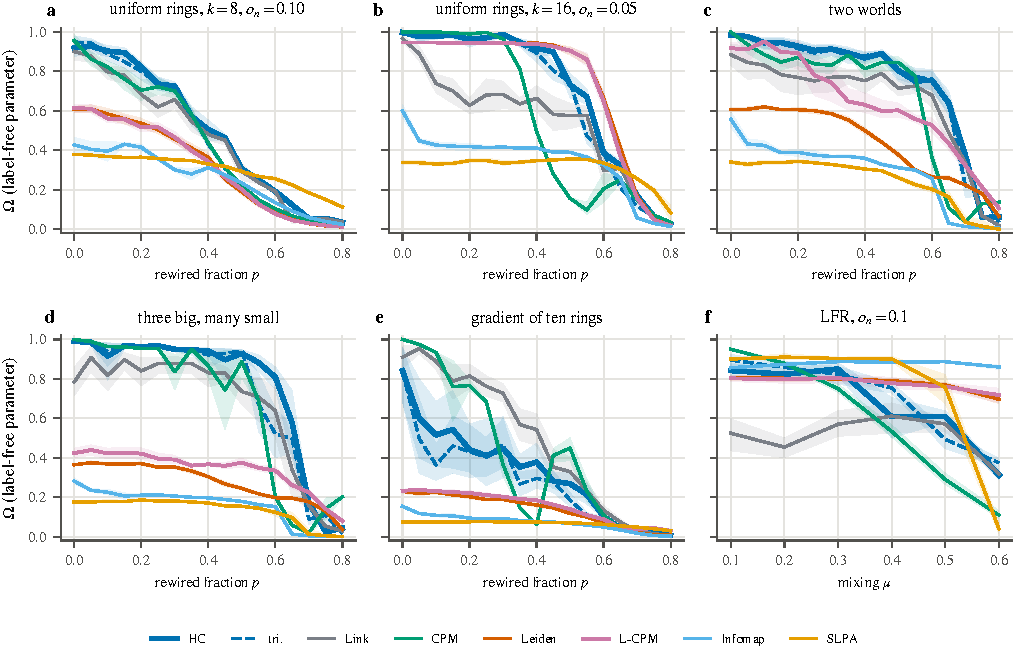
\includegraphics[width=\textwidth]{figures/fig_benchmarks.pdf}
  \caption{Accuracy against noise with every method's parameter chosen without labels
  (largest overlapping modularity on each graph); lines are means over ten test graphs
  and bands 95\% bootstrap intervals. (a,b)~Uniform rings; (c--e)~rings of unequal size
  and density ($o_n=0.05$); (f)~overlapping LFR graphs, against the mixing parameter. In
  (e) the selector picks too fine a cover for HyperCommon (Sec.~\ref{sec:planted}).
  OSLOM and the stochastic block model are not drawn; on the family of (f) OSLOM is the
  most accurate method (Table~\ref{tab:labelfree}). The same panels under the oracle
  protocol are in Fig.~\ref{fig:benchmarksoracle}.}
  \label{fig:benchmarks}
\end{figure*}

Table~\ref{tab:scorecard} summarises the benchmarks. Without labels, over the 28 ring
settings HyperCommon has the highest $\Omega$ in 15, by paired 95\% intervals that
exclude zero, is level with the best other method in 6 and trails in 7: on dense rings
with little overlap, where Leiden leads ($0.84$ against $0.78$ at $k=16$, $o_n=0$), on
rings of equal size and unequal degree at $o_n=0.10$, and on the gradient, where link
communities lead. The margins are largest where community sizes differ and communities
overlap: $\Omega=0.78$ against $0.68$ for clique percolation on three big, many small,
and $0.76$ against $0.66$ on two worlds [Fig.~\ref{fig:benchmarks}(c,d)].

Part of these margins lies in the selector rather than in the objectives. At its best
resolution the Constant Potts Model reaches $0.71$ on three big, many small and $0.78$ on
two worlds, against $0.34$ and $0.64$ when modularity chooses its resolution, while
HyperCommon goes from $0.80$ to $0.78$ and from $0.78$ to $0.76$. Two checks bound this
effect. At each method's own default or selection rule (native protocol), HyperCommon
is still ahead in 17 of the 28 settings, although the Constant Potts Model at the edge
density is then level with it on two worlds with overlap. With the best parameter on
every graph (oracle), every method narrows the gap: HyperCommon is ahead in 11, level in
4 and behind in 13, mostly behind one of the two Leiden objectives, and stays ahead on
three big, many small at every overlap level ($0.80$ against $0.72$ for link communities)
and on the gradient with overlap. Modularity with a single resolution fails on the
gradient even without noise ($\Omega=0.28$ for Leiden, against $0.99$ for HyperCommon),
because small rings are merged while large ones are
split~\cite{fortunato2007resolution,lancichinetti2011limits}. With one parameter frozen
per family, HyperCommon leads in only 1 setting: its best threshold moves with noise, so
one threshold fits the noise-free graphs or the noisy ones but not both. On the gradient
the label-free selector errs the other way, picking too fine a cover ($181$ communities
against $147$ at the best threshold and $10$ planted).

Omega is dominated by the largest communities. On two worlds and three big, many small,
HyperCommon recovers the large rings best but splits the small sparse ones, which the
Constant Potts Model recovers best ($0.53$--$0.54$ against $0.33$--$0.38$;
Tables~\ref{tab:recsmall} and~\ref{tab:reclarge}), so with labels the Constant Potts
Model leads there by ONMI. Over the 28 ring settings HyperCommon leads by ONMI on 10 with
labels and on 15 without (Tables~\ref{tab:onmi-oracle} and~\ref{tab:onmi-label-free}).
Without labels its accuracy also decays latest with noise, or within $0.01$ of the
latest, in ten of the sixteen ring families (Table~\ref{tab:robust}).

\subsection{Ablations}
\label{sec:ablations}

Testing the third, non-adjacent pair of a wedge matters most: without it $\Omega$ falls
in all 36 benchmark settings under the oracle and the label-free protocol, by
$0.06$--$0.34$ on rings and up to $0.42$ on LFR graphs, because a wedge whose two edges
pass reaches into another community whenever its centre has a neighbour there. Admitting
open wedges improves on triangles alone in 26 and 25 of the 36 settings under the two
protocols, most where triangles are scarce ($0.04$--$0.11$ on sparse rings). Joining
triples only through shared edges changes $\Omega$ by at most $0.02$ on the rings when the
parameter is chosen per graph and is slightly better on most LFR families; we keep
joins through non-adjacent pairs because they give Corollary~\ref{cor:pairdisjoint}.
Link communities, whose edge similarity is the commonality of the wedge's third pair,
are less accurate than HyperCommon in 25 of the 28 ring settings under both protocols;
the edge tests separate the two most where communities overlap. Among the commonality
functions, Jaccard is the best, or within $0.01$ of it, on seventeen of eighteen
benchmark settings with the best threshold (Tables~\ref{tab:familyoracle}
and~\ref{tab:familyfree}).

\subsection{Where it breaks: LFR graphs and random communities}
\label{sec:geometry}

\begin{table*}[t]
\caption{Internal geometry: before the noise, a fraction $q$ of each ring's edges is rewired inside the ring, from lattice rings ($q=0$) to rings that are random graphs ($q=1$), at fixed size and mean degree; $o_n=0.05$. Uniform: 40 rings of 50 nodes, $k=8$; two worlds: five rings of 200 nodes ($k=32$) and twenty of 50 ($k=8$); three big, many small: three of 400 ($k=32$) and sixteen of 50 ($k=8$); gradient: ten rings of 600 to 30 nodes ($k=16$ to 8). Mean $\Omega$ over $p\in\{0,0.1,\dots,0.6\}$, ten test graphs per noise level, under the oracle and label-free protocols, for HyperCommon (HC), its triangles-only variant and the best other method; $C$: mean clustering of the noiseless graphs (ten seeds); cov.: coverage of HC's label-free cover. Superscripts on HC: paired 95\% interval of its difference from the best other method excludes zero ($^+$ HC ahead, $^-$ behind). Bold: HC best or within 0.005 of the best other method. Means are over $p\in\{0,0.1,\dots,0.6\}$, so the $q=0$ entries differ from those of Tables~\ref{tab:labelfree} and~\ref{tab:oracle} for the same families, which average over $p\in[0,0.8]$.}
\label{tab:geometry}
\footnotesize\setlength{\tabcolsep}{3pt}
\begin{ruledtabular}
\begin{tabular}{lcccccccccc}
 & & & \multicolumn{3}{c}{oracle} & \multicolumn{4}{c}{label-free} \\
Family & $q$ & $C$ & HC & tri. & best other & HC & tri. & best other & cov. \\
\hline
uniform, $k{=}8$ & 0.0 & 0.62 & \textbf{0.73$^+$} & 0.65 & 0.73 (Link) & \textbf{0.70$^+$} & 0.64 & 0.67 (Link) & 0.98 \\
 & 0.1 & 0.48 & 0.68$^-$ & 0.56 & 0.81 (Leiden) & 0.65 & 0.56 & 0.66 (Leiden) & 0.97 \\
 & 0.3 & 0.28 & 0.62$^-$ & 0.41 & 0.85 (Leiden) & 0.57$^-$ & 0.41 & 0.74 (Infomap) & 0.95 \\
 & 0.6 & 0.16 & 0.61$^-$ & 0.28 & 0.86 (Leiden) & 0.55$^-$ & 0.28 & 0.77 (Infomap) & 0.96 \\
 & 1.0 & 0.15 & 0.60$^-$ & 0.29 & 0.85 (Leiden) & 0.55$^-$ & 0.28 & 0.78 (Infomap) & 0.95 \\
\hline
two worlds & 0.0 & 0.67 & \textbf{0.91} & 0.90 & 0.91 (L-CPM) & \textbf{0.89$^+$} & 0.89 & 0.82 (CPM) & 0.94 \\
 & 0.1 & 0.51 & 0.88$^-$ & 0.87 & 0.94 (L-CPM) & 0.86$^-$ & 0.86 & 0.91 (L-CPM) & 0.93 \\
 & 0.3 & 0.30 & 0.84$^-$ & 0.81 & 0.95 (L-CPM) & 0.82$^-$ & 0.80 & 0.92 (L-CPM) & 0.94 \\
 & 0.6 & 0.17 & 0.72$^-$ & 0.68 & 0.95 (L-CPM) & 0.69$^-$ & 0.66 & 0.92 (L-CPM) & 0.91 \\
 & 1.0 & 0.16 & 0.66$^-$ & 0.66 & 0.95 (L-CPM) & 0.62$^-$ & 0.66 & 0.92 (L-CPM) & 0.92 \\
\hline
three big, many small & 0.0 & 0.68 & \textbf{0.94$^+$} & 0.93 & 0.87 (CPM) & \textbf{0.93$^+$} & 0.91 & 0.85 (CPM) & 0.90 \\
 & 0.1 & 0.51 & 0.92$^-$ & 0.91 & 0.95 (L-CPM) & \textbf{0.91$^+$} & 0.91 & 0.83 (CPM) & 0.91 \\
 & 0.3 & 0.28 & 0.84$^-$ & 0.80 & 0.96 (L-CPM) & 0.83$^-$ & 0.79 & 0.95 (L-CPM) & 0.91 \\
 & 0.6 & 0.13 & 0.51$^-$ & 0.61 & 0.96 (L-CPM) & 0.50$^-$ & 0.56 & 0.95 (L-CPM) & 0.83 \\
 & 1.0 & 0.11 & 0.28$^-$ & 0.54 & 0.96 (L-CPM) & 0.27$^-$ & 0.45 & 0.95 (L-CPM) & 0.80 \\
\hline
gradient of ten rings & 0.0 & 0.66 & \textbf{0.74$^+$} & 0.72 & 0.70 (Link) & 0.42$^-$ & 0.37 & 0.64 (Link) & 0.93 \\
 & 0.1 & 0.49 & 0.65$^-$ & 0.63 & 0.73 (L-CPM) & 0.43$^-$ & 0.38 & 0.55 (Link) & 0.93 \\
 & 0.3 & 0.25 & 0.44$^-$ & 0.43 & 0.86 (L-CPM) & 0.40$^-$ & 0.34 & 0.76 (Walktrap) & 0.93 \\
 & 0.6 & 0.08 & 0.16$^-$ & 0.11 & 0.88 (L-CPM) & 0.16$^-$ & 0.09 & 0.86 (L-CPM) & 0.87 \\
 & 1.0 & 0.04 & 0.11$^-$ & 0.02 & 0.87 (L-CPM) & 0.09$^-$ & 0.01 & 0.85 (L-CPM) & 0.89 \\
\end{tabular}
\end{ruledtabular}
\end{table*}


HyperCommon trails on all eight LFR families under every protocol; OSLOM is the most
accurate method on most of them without labels. The pairwise signal is not what fails:
the AUC of the commonality of edges inside against across planted communities is $0.97$
at $\mu=0.3$, and wedges spanning two communities pass the three-pair test at $t=0.1$
with probability below $10^{-4}$. What fails is connectivity inside large communities.
LFR communities are random graphs internally, with degree independent of size, so a
large community is sparse and its members share few neighbours: at $\mu=0.3$, $89\%$ of
the wedges inside communities of at most 40 nodes pass at $t=0.1$, but only $21\%$ of
those inside communities of at least 80 nodes. Percolation then breaks large
communities into pieces at any threshold that keeps communities apart, which is why the
deficit is largest with large communities ($0.42$ against $0.89$ for OSLOM).

The geometry families test this directly (Table~\ref{tab:geometry}): sizes, degrees and
overlap are fixed while a fraction $q$ of each ring's edges is rewired inside the ring,
so adjacent members go from sharing up to $k-2$ neighbours to sharing about
$(k-1)^2/s$. On lattice communities HyperCommon is ahead of every other method with
labels in three of the four families and level in the fourth. With labels the advantage
is gone once a tenth of each community's edges are rewired, while the communities are
still strongly clustered; without labels it holds on three big, many small at $q=0.1$;
from $q=0.3$ on the best other method is ahead everywhere. Degree-preserving swaps give
the same result within $0.01$ at $q=0.1$ and $0.3$, so the change of degrees is not the reason. The controls
(Table~\ref{tab:S-controls}) point the same way: hubs inside the rings move
HyperCommon's $\Omega$ by at most $0.03$, splitting the edges of shared nodes as in LFR
graphs by at most $0.05$, and random geometric communities, clustered but not lattices,
leave it behind the best other method with labels. On clustered graphs with no planted
communities every method reports communities, HyperCommon $101$ and $175$
(Table~\ref{tab:S-nulls}), so a cover it returns is not by itself evidence of community
structure.

\subsection{Real networks}
\label{sec:real}

\begin{table*}[t]
\caption{Detection on the full SNAP Amazon (334\,863 nodes), DBLP (317\,080) and YouTube (1\,134\,890) graphs, scored on the nodes of their ground-truth communities (top 5000 for Amazon and DBLP, all groups of at least three nodes for YouTube), to which every detected community is restricted. Best-match F1 against the recorded communities and $\Omega$ against their distinct node sets, at each method's best parameter by that metric (best) and at the parameter chosen without labels by maximal overlapping modularity on the full graph (free); cov.: fraction of the scored nodes in at least one community at the free parameter. HC$_f$: the seven commonality functions together, the free choice taken over all of them. Leiden at $\gamma=1$ and Infomap at Markov time 1 are the two methods at their defaults (one parameter, so best and free coincide). Connected components are a trivial reference. On YouTube HyperCommon uses degree-ratio pruning, exact for every $t\ge0.02$ (Sec.~\ref{sec:cost}), which excludes link communities and the other functions; clique percolation and SLPA are compared on the induced subgraphs (Table~\ref{tab:realinduced}), and SCAN, Walktrap, DEMON and ANGEL were not run on these graphs, to bound the computing time of the large runs. Stochastic methods: one seed. F1 against the distinct node sets is in Table~\ref{tab:S-realnet-dedup}; it changes F1 by at most 0.03 (at most 0.01 for HyperCommon and its variants) and reverses the order of no two methods in a column. The top-5000 lists of Amazon and DBLP frequently consist of near-cliques~\cite{chen2024parallel}, which can favour methods that find small dense groups. Bold: best in column.}
\label{tab:real}
\scriptsize\setlength{\tabcolsep}{2pt}
\begin{ruledtabular}
\begin{tabular}{lccccccccccccccc}
 & \multicolumn{5}{c}{Amazon} & \multicolumn{5}{c}{DBLP} & \multicolumn{5}{c}{YouTube} \\
 & F1 best & F1 free & $\Omega$ best & $\Omega$ free & cov. & F1 best & F1 free & $\Omega$ best & $\Omega$ free & cov. & F1 best & F1 free & $\Omega$ best & $\Omega$ free & cov. \\
\hline
components & 0.020 & 0.020 & 0.000 & 0.000 & 1.00 & 0.075 & 0.075 & 0.000 & 0.000 & 1.00 & 0.060 & 0.060 & 0.000 & 0.000 & 1.00 \\
HC & 0.856 & 0.854 & 0.459 & 0.459 & 0.99 & 0.516 & 0.486 & 0.024 & 0.024 & 0.94 & 0.322 & 0.289 & 0.017 & $-0.007$ & 0.67 \\
HC$_f$ & 0.884 & 0.852 & 0.477 & 0.477 & 1.00 & 0.520 & 0.486 & 0.037 & 0.024 & 0.94 & -- & -- & -- & -- & -- \\
e-conn. & 0.857 & 0.857 & 0.485 & 0.485 & 0.99 & 0.516 & 0.487 & 0.024 & 0.024 & 0.94 & 0.323 & 0.292 & 0.016 & $-0.007$ & 0.67 \\
tri. & 0.840 & 0.838 & 0.415 & 0.415 & 0.95 & 0.513 & 0.485 & 0.030 & 0.019 & 0.89 & 0.309 & 0.300 & 0.015 & 0.006 & 0.49 \\
2-test & 0.887 & 0.887 & 0.424 & 0.424 & 0.95 & 0.507 & 0.459 & 0.014 & 0.014 & 0.83 & 0.280 & 0.215 & 0.005 & $-0.011$ & 0.53 \\
Link & 0.842 & 0.827 & 0.487 & 0.487 & 1.00 & 0.490 & 0.446 & 0.031 & 0.024 & 1.00 & -- & -- & -- & -- & -- \\
Leiden & 0.924 & 0.534 & 0.600 & 0.392 & 1.00 & 0.542 & 0.285 & \textbf{0.154} & \textbf{0.152} & 1.00 & \textbf{0.363} & 0.192 & \textbf{0.142} & 0.074 & 1.00 \\
Leiden, $\gamma{=}1$ & 0.534 & 0.534 & 0.392 & 0.392 & 1.00 & 0.285 & 0.285 & 0.152 & \textbf{0.152} & 1.00 & 0.192 & 0.192 & 0.074 & 0.074 & 1.00 \\
L-CPM & 0.929 & 0.561 & \textbf{0.617} & 0.385 & 1.00 & 0.532 & 0.237 & 0.150 & 0.150 & 1.00 & 0.337 & 0.252 & 0.113 & 0.104 & 1.00 \\
Infomap & \textbf{0.935} & 0.900 & 0.583 & \textbf{0.583} & 1.00 & 0.545 & 0.518 & 0.042 & 0.029 & 1.00 & 0.355 & \textbf{0.337} & 0.126 & \textbf{0.126} & 1.00 \\
Infomap, Markov time 1 & 0.918 & \textbf{0.918} & 0.488 & 0.488 & 1.00 & 0.545 & \textbf{0.545} & 0.013 & 0.013 & 1.00 & 0.337 & \textbf{0.337} & 0.126 & \textbf{0.126} & 1.00 \\
LPA & 0.820 & 0.820 & 0.373 & 0.373 & 1.00 & 0.508 & 0.508 & 0.010 & 0.010 & 1.00 & 0.216 & 0.216 & 0.007 & 0.007 & 1.00 \\
OSLOM & 0.882 & 0.834 & 0.560 & 0.536 & 1.00 & \textbf{0.549} & 0.351 & 0.028 & 0.028 & 1.00 & 0.338 & 0.253 & 0.125 & 0.125 & 1.00 \\
\end{tabular}
\end{ruledtabular}
\end{table*}


Table~\ref{tab:real} reports detection on the full Amazon, DBLP and YouTube
graphs~\cite{yang2015defining}. HyperCommon's threshold is chosen without labels at
little cost: the label-free F1 is $99.9\%$, $94\%$ and $89\%$ of its best F1. The same
selector serves the modularity-based methods less well: Leiden falls to $0.53$, $0.29$
and $0.19$ in F1, about half of its best values. Under this selector Infomap is the most
accurate on all three graphs (F1 $0.90$, $0.52$ and $0.34$), with label-free
HyperCommon within $0.03$--$0.05$; by $\Omega$ the modularity- and flow-based partitions
lead.

Table~\ref{tab:realmore} of the Supplemental Material extends the comparison to fourteen
smaller networks from the
Netzschleuder repository~\cite{peixoto2020netzschleuder}: ten Facebook ego networks with
their users' own social circles~\cite{mcauley2012learning}, college football
conferences~\cite{girvan2002community}, political books~\cite{krebs_polbooks,newman2006modularity}
and blogs~\cite{adamic2005political}, and the classes of a primary
school~\cite{stehle2011high}. With its best threshold HyperCommon is the most accurate on
college football and within $0.01$ of the best, OSLOM, on political blogs; its mean rank
among seventeen methods is $8.9$ without labels and $8.1$ with labels, and the most
accurate method varies from network to network~\cite{peel2017ground}. The choice of
commonality function matters here: on the primary school it alone raises F1 from $0.41$
to $0.83$. Testing the third pair helps less than on the benchmarks: with the best
threshold the two-test variant has the higher F1 on nine of the fourteen networks. Over
all seventeen networks the label-free threshold retains a median $94\%$ of the best F1.
